\section{Dataset and Reference Qualification}\label{app:A}
\subsection{Scientific target and sampling unit}
TopoWorld-Eval asks whether an AI can maintain one grounded spatial world across views, tasks, and later evidence changes. A successful response should refer to the same physical instances across drawings, realize the supported spatial relations in executable geometry, avoid represented material conflicts, and revise evidence-dependent claims when a source changes. These requirements are related, but success on one does not establish success on the others.

The primary static material consists of public architectural drawings for 14 physical buildings. Twelve buildings occur in both the original semantic-locator condition v1 and its neutral-locator control N2. Two further complex-staircase buildings occur in CS1. Thus v1 plus N2 does not provide 24 independent buildings. The repeated conditions instead provide controlled comparisons on the same visual material. Likewise, eight configurations and several queries per building increase the number of observations without increasing the number of sampled buildings.

The material supports bounded target-fragment evaluation. It does not require reconstruction of every wall or opening in a complete building. Targets concentrate on floor relationships, doors and windows, staircase endpoints, and identity across drawing views. The sample includes schools, houses, civic buildings, missions, and institutional quarters. It was assembled for these structural questions rather than drawn as a random sample of all architecture. The empirical conclusions therefore concern the observed buildings and task conditions.

\subsection{Building and drawing inventory}
Table~\ref{tab:A-catalogue} identifies all buildings. The 12 N2 cases contain 35 pages, rendered at a 3,200-pixel long side. CS1 adds seven pages at a 3,000-pixel long side. Original source identifiers, public page URLs, image dimensions, and SHA-256 values are preserved in the package catalogue. View identifiers were shuffled in N2; the catalogue retains the mapping to the source page.

\begin{table}[htbp]\centering\small
\begin{tabular}{p{.20\linewidth}p{.57\linewidth}r}
\toprule Case & Building / source collection & Pages\\\midrule
A01 & Octagon House, Washington DC; HABS DC-25 & 3\\
A02 & Drayton Hall, South Carolina; HABS SC-377 & 3\\
A06 & Octagon House, Watertown; HABS WI-135 & 3\\
B01 & Westside School, Las Vegas; NV0473 & 3\\
B02 & Madison County Courthouse, Virginia City; MT0028 & 3\\
B03 & San Xavier del Bac Mission, Tucson; AZ0061 & 3\\
B04 & Mission San Luis Obispo Monastery; CA0801 & 3\\
B05 & Mission Frame House, Honolulu; HI0032 & 3\\
B06 & William Scarborough House, Savannah; GA0030 & 3\\
C01 & Quarters No. 211, San Juan; PR0070 & 3\\
C02 & Rock Schoolhouse, Fillmore; UT0027 & 2\\
C03 & Idaho City Schoolhouse; HABS ID-6 & 3\\\midrule
CS1--S01 & Lovell Health House; HABS CA-1936 & 3\\
CS1--S02 & Gamble House; HABS CA-1981 & 4\\\bottomrule
\end{tabular}
\caption{The 14 physical buildings and 42 whole-page drawings. Short case IDs are expanded to their stable package IDs in the catalogue. v1 and N2 reuse the first 12 buildings.}\label{tab:A-catalogue}
\end{table}

Public availability and a source citation do not by themselves establish a blanket redistribution license for every archival item. The package retains the Library of Congress source and rights information where supplied. Private Loft photographs and account information are excluded. Historical Loft examples in the casebook use reconstructed coordinates and diagnostic diagrams, not private image files.

\subsection{Reference obligations and evidence isolation}
The fixed list contains 96 relation obligations: 95 determinate values and one explicitly unresolved identity. N2 contributes 75 determinate values and one unknown; CS1 contributes 20 determinate values. Across the 95 determinate obligations, 71 are TRUE and 24 are FALSE. The predicate distribution appears in Table~\ref{tab:A-predicates}. Queries are frozen obligations, not relations selected after seeing an output. Some require several pages; others concern multiple drawings on one sheet.

\begin{table}[htbp]\centering
\begin{tabular}{lr@{\qquad}lr}\toprule
Predicate & Count & Predicate & Count\\\midrule
\texttt{connected\_by} & 4 & \texttt{same\_floor} & 11\\
\texttt{above} & 14 & \texttt{window\_host} & 17\\
\texttt{identity\_assignment} & 23 & \texttt{door\_host} & 8\\
\texttt{disjoint} & 9 & \texttt{stair\_connects} & 10\\\bottomrule
\end{tabular}
\caption{All 96 obligations, including the one unresolved identity. Types are not equally frequent or equally difficult.}\label{tab:A-predicates}
\end{table}

Each reference record identifies the query, arguments, frozen value, source page, and supporting explanation. The audit also links approximate crops and target points for human review. These review crops are derivatives; they were not additional model inputs. The reference geometry is not a unique coordinate model. When several geometric completions can express the same supported relation, the benchmark allows them rather than requiring a hidden metric reconstruction.

The reference list and the model input are separate objects. R and A do not receive organizer relation answers. B deliberately receives the determinate relation values as a controlled input. It receives neither hidden reference coordinates nor the organizer's localization boxes. B therefore measures construction with relation assistance. It cannot be described as unaided image reconstruction.

Reference records retain their historical AI-assisted annotation metadata. Later, the author explicitly confirmed personally checking all 96 relations. The completion record preserves this statement without changing the frozen values. No separate per-item verdict file or second expert's review was supplied. Accordingly, the correct qualification is author-reviewed, AI-assisted reference construction. Inter-annotator agreement and independent expert certification have not been measured.

\subsection{How to inspect a reference}
A reviewer can start with a query row, open its listed public page, locate its target point, and then inspect the indicated source region. For an identity query, both observations must be checked. A repeated printed label can be a component type rather than a physical instance. For a staircase, the review must distinguish the whole assembly, a run, a landing, and a nearby space. The question must also refer to a supported granularity: the endpoint of a two-riser transition is not necessarily the endpoint of a complete multi-floor staircase.

The evidence table records what the drawing supports and what remains unknown. It does not infer a removed wall from an omitted drafting line, public access from physical contact, or physical identity from equal labels. If a source is a historical plan and another page represents a different state, matching image position is insufficient to assert that an opening is the same surviving object.

The single unresolved case is B04's cross-era identity. The selected pages do not establish whether the two observations are one persisting physical instance. UNKNOWN is the supported epistemic answer. A definite SAME answer is unsupported certainty; it is not necessarily a proven false statement about the actual building. This distinction matters when interpreting the low uncertainty score in Appendix~\ref{app:G}.

\begin{figure}[htbp]\centering
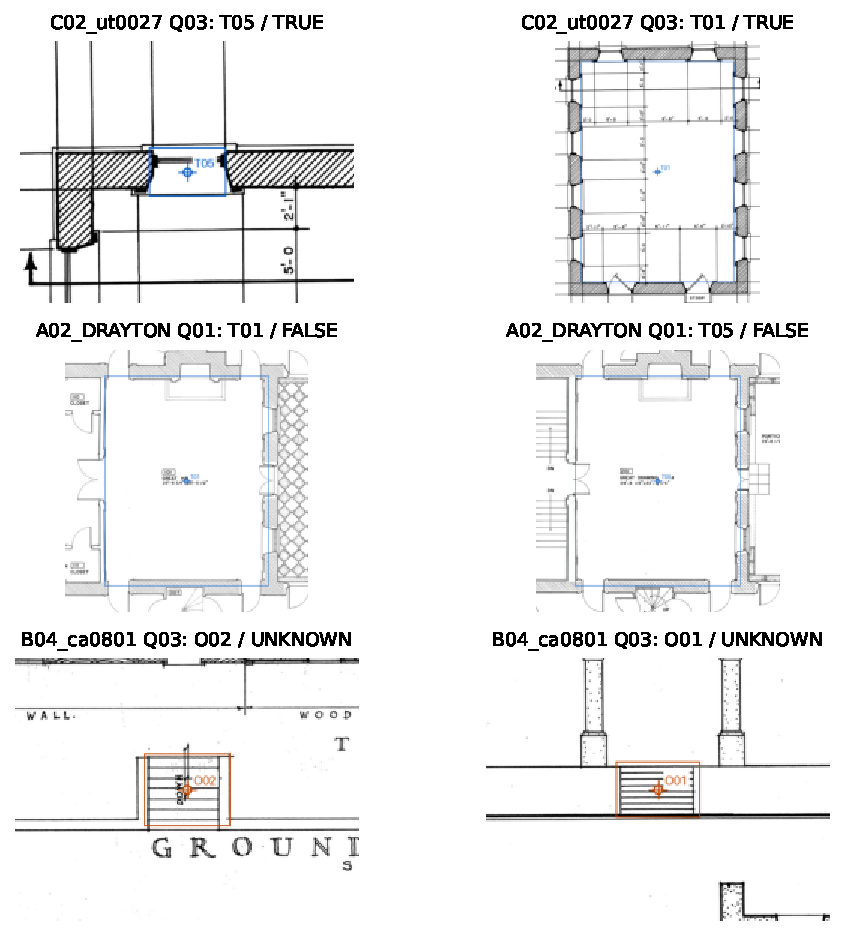
\includegraphics[width=.94\linewidth]{figures/reference_evidence.pdf}
\caption{Three source-to-reference examples: an opening incident to its classroom, two spaces on different floors, and a cross-era identity that remains unresolved. These organizer-review crops show the reference regions, not model boxes. Public page IDs and parent hashes are retained; the models received full assigned pages.}\label{fig:A-reference}
\end{figure}

\subsection{Controls on task difficulty and label imbalance}
N2 removes semantic identifiers such as named floors or room labels from organizer-provided target names. It replaces them with arbitrary T/O identifiers, shuffled V identifiers, point locators, and optional class hints. Text actually printed in an image remains available. The control therefore reduces organizer-supplied answer cues while retaining a feasible given-point localization task. It is not unprompted object discovery.

CS1 adds complex staircase cases and explicit granularity hints. These hints identify what assembly or local step transition is queried; they do not supply the answer or a correct coordinate model. CS1 also balances its determinate values, with ten TRUE and ten FALSE. It is a separate two-building challenge set, not an estimate of prevalence across all complex buildings.

For N2 alone, a constant TRUE predictor obtains 61/75, or 81.33\%. This simple diagnostic makes the label skew visible. It cannot construct a world, localize objects, or explain an identity. Still, it is a necessary reference when interpreting a high direct-answer percentage. Balanced CS1 and predicate-specific results help show which parts of the task exceed this shortcut.

The evaluation tasks were frozen before their respective model allocations. The study does not claim all drawings were unknown to model pretraining. The controls concern exposure through this experiment, not unverifiable historical training data. Future data collection should add independently qualified buildings and further uncertainty cases rather than treating more questions on the current drawings as new buildings.
